\documentclass[hyperref={unicode}]{beamer}
\usetheme{Madrid}
\usepackage[utf8]{inputenc}
\usepackage[czech]{babel}
\usepackage{csquotes}
\usepackage{animate}
\usepackage{amsmath}
\usepackage{amssymb}
\usepackage{ragged2e}
\usepackage[czech, ruled, linesnumbered, noline, longend]{algorithm2e}
\usepackage{biblatex}
\addbibresource{zdroje.bib}
\usepackage{graphicx}

\title{Borůvkův algoritmus}
\author{Richard Klem}

\date{\today}
\begin{document}
\maketitle
\begin{frame}{Obsah}
\begin{itemize}
\item Definice problému
\item Trocha z histrorie
\item Pseudokód
\item Složitost algoritmu
\item Příklad
\end{itemize}
\end{frame}
\begin{frame}{Definice problému}
\framesubtitle{Definice pojmů}
    \begin{block}{Kostra grafu}
    Nechť $G=(V_G,E_G)$ je graf definovaný množinou vrcholů $V_G$ a množinou hran $E_G$.\\
    Pak podgraf $F=(V_F,E_F)$, takový, že $V_F=V_G$, $E_F \subseteq E_G$ a $F$ je stromem, je kostrou grafu $G$.
    \end{block}
    \begin{block}{Minimální kostra}
    Minimální kostra $F$ grafu $G=(V_G,E_G)$, je taková kostra, kde hrany $e \in E_G$ jsou ohodnoceny nějakým číslem a součet hodností hran kostry $$\sum\limits_{e\in E_F}w(e)$$, kde $w(e)$ je hodnost hrany, je minimální.
    \end{block}
\end{frame}


\begin{frame}{Definice problému}
\framesubtitle{Borůvkův algoritmus}
Borůvkův algoritmus řeší problém hledání nejmenší kostry grafu.\\
Algoritmus pracuje s grafy, které mají ohodnocení hran pomocí nezáporných čísel.
\end{frame}
\begin{frame}
\frametitle{Pseudokód}
\textsc{Borůvkůkv algoritmus}
\IncMargin{1.5em}
\begin{algorithm}[H]
{\small
    \KwIn{Graf $G = (V_G, E_G)$ s různě a nezáporně ohodnocenými hranami.\\
    \quad\quad\quad$C_{old} = {V_G}$, $C_{new}=\{\}$, $E_F=\{\}$.}
    \KwOut{Minimální kostra $F=(V_G, E_F)$.}
    \While{$|C_{old}| > 1$}{
        \ForEach{komponenta v $C_{old}$}{
            Najdi hranu vedoucí z komponenty s nejmenším ohodnocením.\\
            Zjisti do které komponenty hrana vede.\\
            Z těchto dvou komponent vytvoř jednu novou.\\
            \If{Nová komponenta ještě v $C_{new}$ není}
            { 
                Do $C_{new}$ vlož tuto nově vytvořenou  komponentu.\\
                Do $E_F$ vlož vybranou hranu.
            }
        }
        $C_{old}=C_{new}$
    }
}
\end{algorithm}
\end{frame}
\begin{frame}{Složitost algoritmu}
    \begin{block}{Asymptotická složitost}
    Asymtotická časová složitost algoritmu vyjadřuje vztah mezi velikostí vstupních dat a potřebným časem pro zprácování tohoto vstupu.
    \end{block}
    \begin{itemize}
    \item<2-> Borůvkův algoritmus s každou iterací sníží počet komponent minimálně na polovinu.
    \item<3-> Algoritmus má tedy logaritmickou složitost $$\mathcal{O}(log(|V|))$$, kde $|V|$ je počet vrcholů grafu.
        
    \end{itemize}
\end{frame}

\begin{frame}{Příklad}
\begin{figure}[H]
    \centering
    \scalebox{0.25}{

    \only<1>{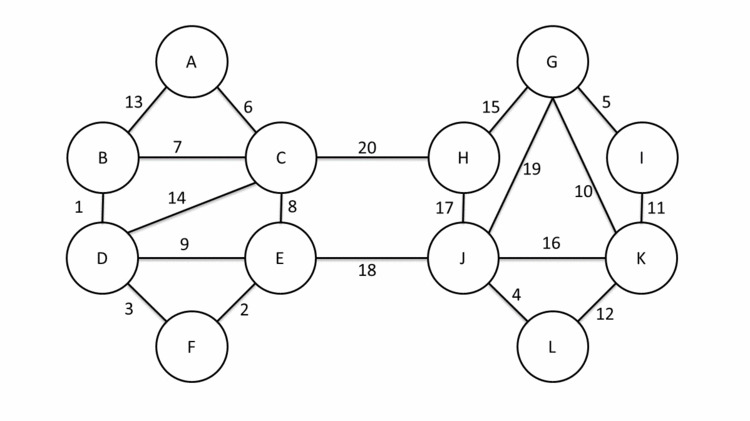
\includegraphics{graph-0.jpg}}}
    \scalebox{0.25}{

    \only<2>{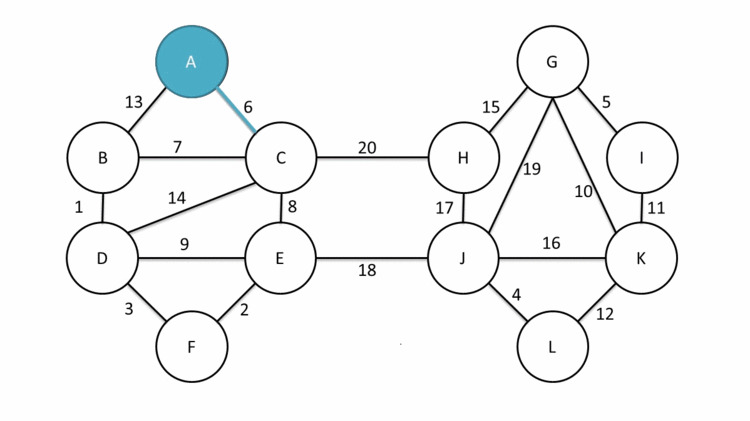
\includegraphics{graph-1.jpg}}}
    \scalebox{0.25}{

    \only<3>{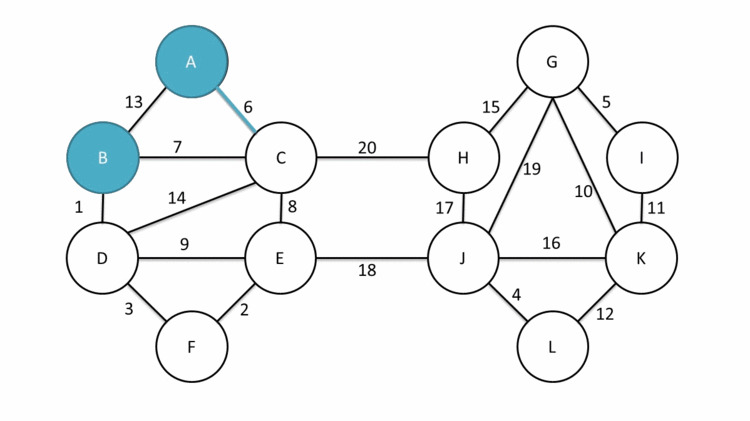
\includegraphics{graph-2.jpg}}}
    \scalebox{0.25}{

    \only<4>{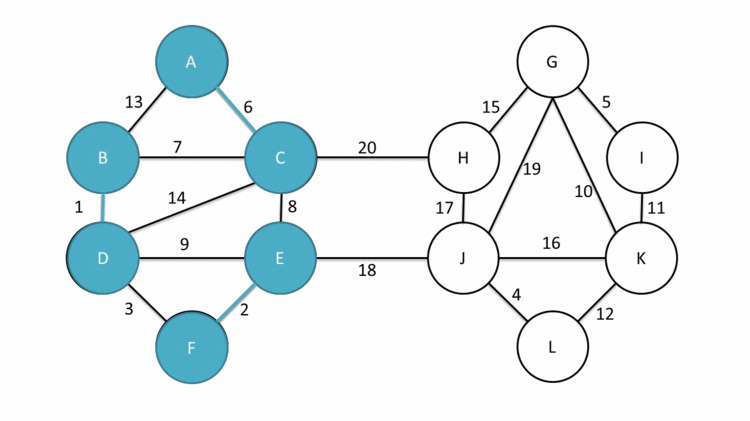
\includegraphics{graph-3.jpg}}}
    \scalebox{0.25}{

    \only<5>{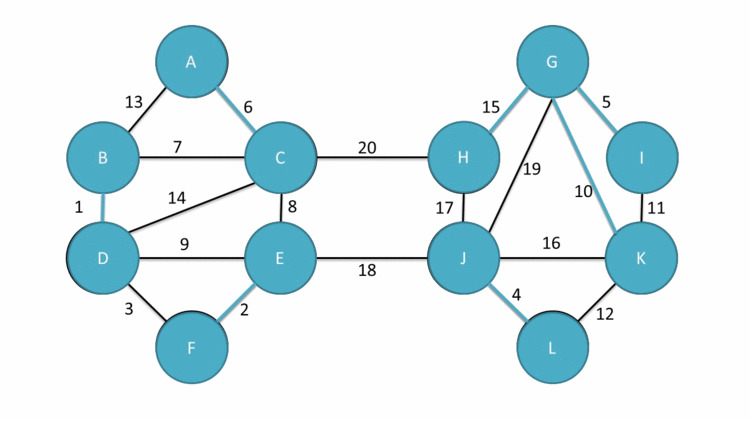
\includegraphics{graph-4.jpg}}}
    \scalebox{0.25}{
    
    \only<6>{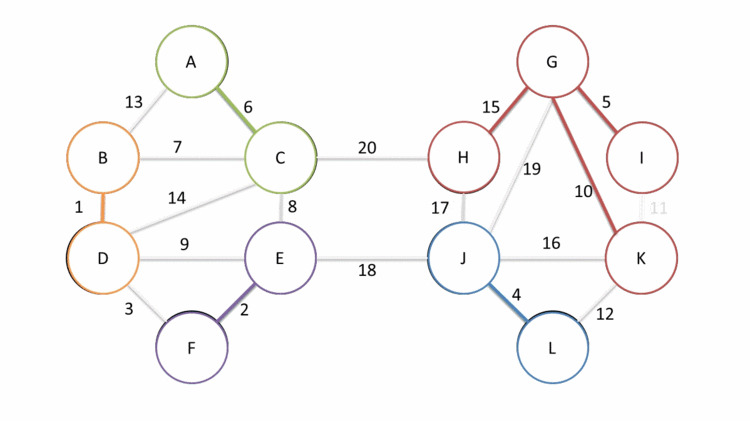
\includegraphics{graph-5.jpg}}}
    \scalebox{0.25}{

    \only<7>{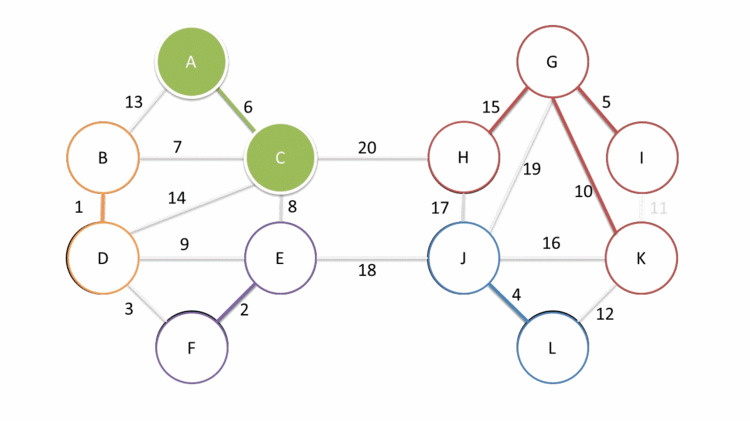
\includegraphics{graph-6.jpg}}}
    \scalebox{0.25}{

    \only<8>{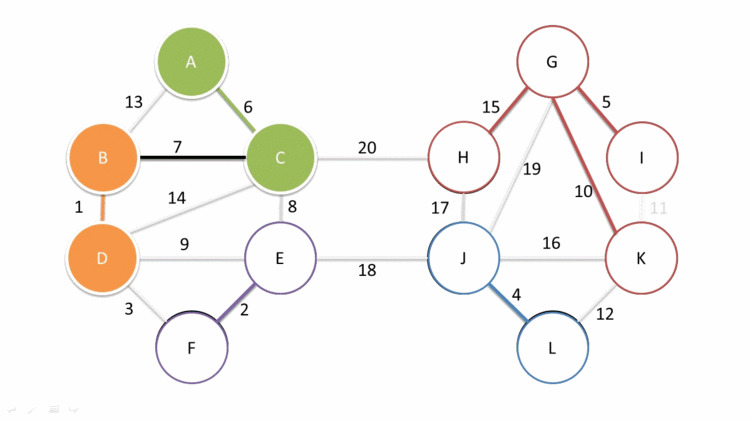
\includegraphics{graph-7.jpg}}}
    \scalebox{0.25}{

    \only<9>{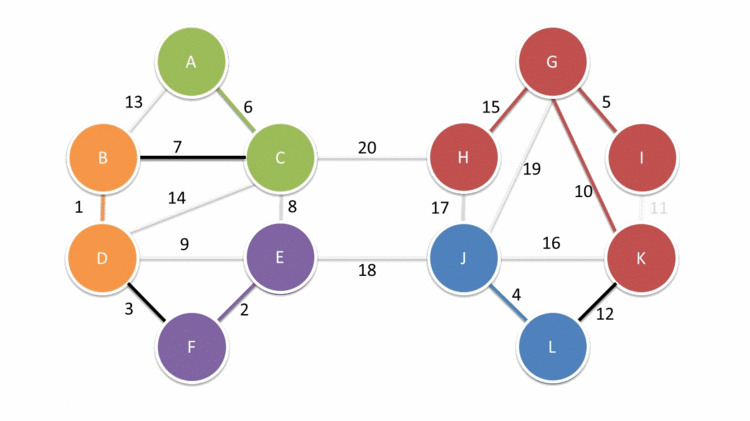
\includegraphics{graph-8.jpg}}}
    \scalebox{0.25}{

    \only<10>{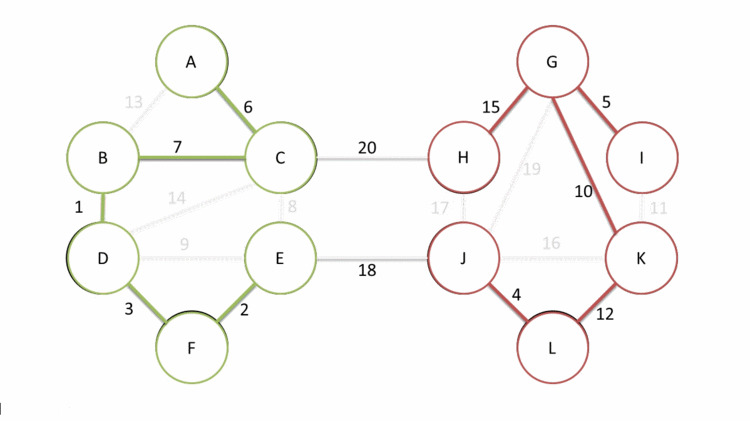
\includegraphics{graph-9.jpg}}}
    \scalebox{0.25}{

    \only<11>{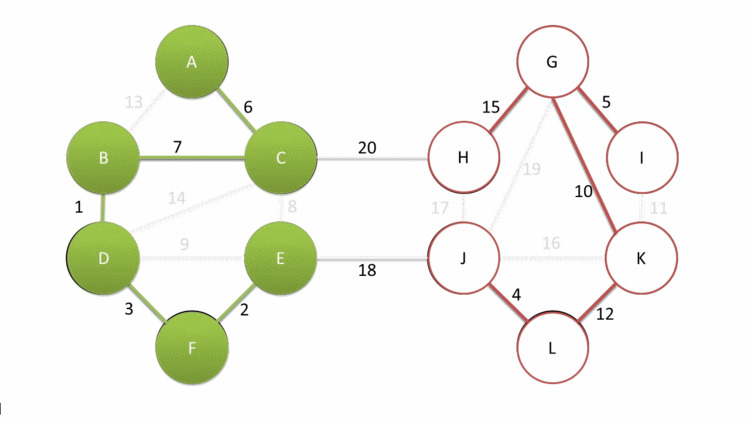
\includegraphics{graph-10.jpg}}}
    \scalebox{0.25}{

    \only<12>{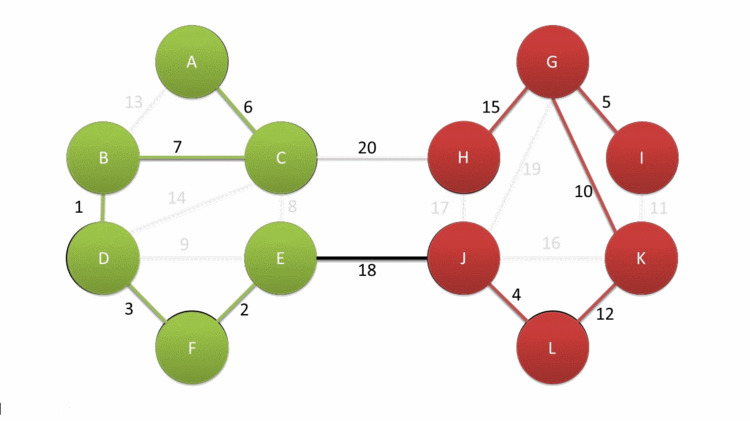
\includegraphics{graph-11.jpg}}}
    \scalebox{0.25}{

    \only<13>{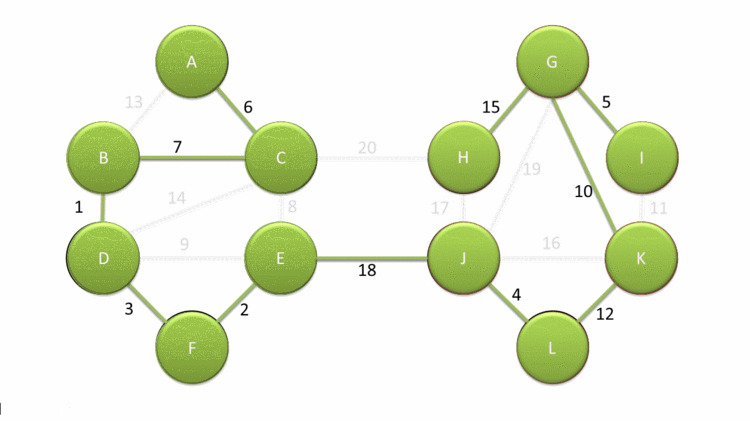
\includegraphics{graph-12.jpg}}}
    \caption{Průběh hledání minimální kostry grafu.\cite{pict}}
\end{figure}
\end{frame}
\begin{frame}{Zdroje}
\printbibliography
\end{frame}
\end{document}
